\begin{frame}[shrink=20]
  \frametitle{Agenda}
  \begin{itemize}
    \item Introducción:
      \begin{itemize}
        \item Aplicaciones web y la seguridad.
        \item Estándares y protocolos.
      \end{itemize}
    \item Situación actual. Estado del arte:
      \begin{itemize}
        \item Soluciones WAF privativas.
        \item Soluciones WAF de software libre.
        \item Comparativa soluciones actuales.
      \end{itemize}
    \item Solución.
      \begin{itemize}
        \item Objetivo.
        \item Diseño.
        \item Arquitectura.
      \end{itemize}
    \item Conclusiones.
    \item Test y resultados.
  \end{itemize}
\end{frame}

\section{Introducción}
\subsection{Aplicaciones web y la seguridad}
\begin{frame}[shrink=20]
  \frametitle{Aplicaciones web y la seguridad}
  \begin{block}{Premisa}
     La seguridad 100\% no existe.
  \end{block}
  Las aplicaciones web están siendo atacadas continuamente.
  \begin{figure}
    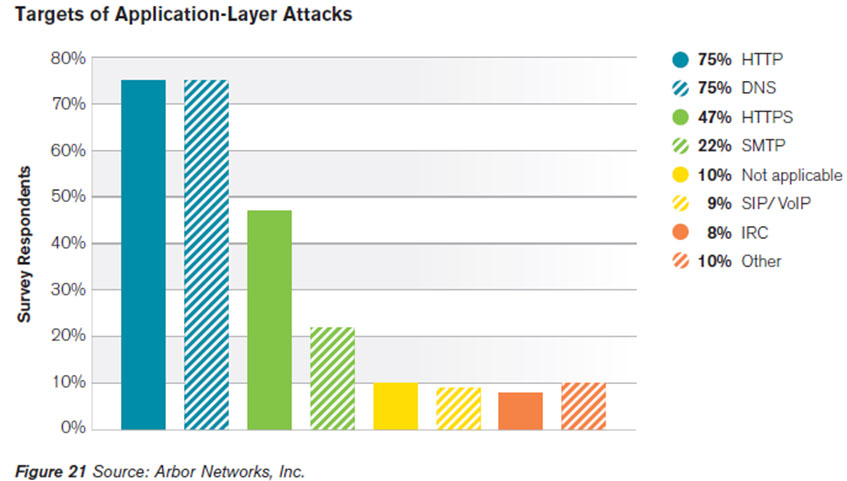
\includegraphics[width=0.35\textwidth]{fig/application-attacks-2}%
    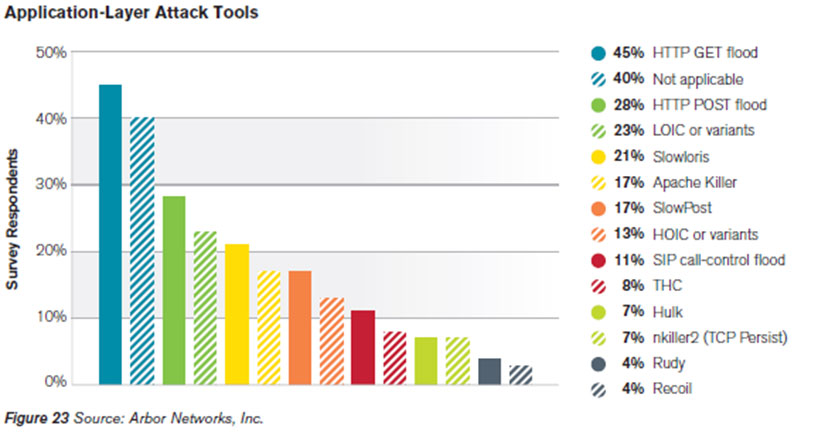
\includegraphics[width=0.35\textwidth]{fig/application-attacks-1}
    \label{fig:applicationattacks}
    \caption{\small{Ataques en capa de aplicación (fuente Arbor~\cite{articleArbor})}}
  \end{figure}
  \begin{alertblock}{Conclusión}
    Se debe realizar un esfuerzo continuo para mejor la seguridad de las plataformas web.
  \end{alertblock}
\end{frame}

\begin{frame}[shrink=20]
  \frametitle{Vulnerabilidades en plataformas web}
	\begin{columns}
	\begin{column}{0.5\textwidth}
		Existen múltiples vulnerabilidades en las plataformas web (referencia {\em \acrlong{owasp}}, \acrshort{owasp}~\cite{owasptop10}).
	\end{column}
	\begin{column}{0.5\textwidth}  %%<--- here
		\begin{figure}
			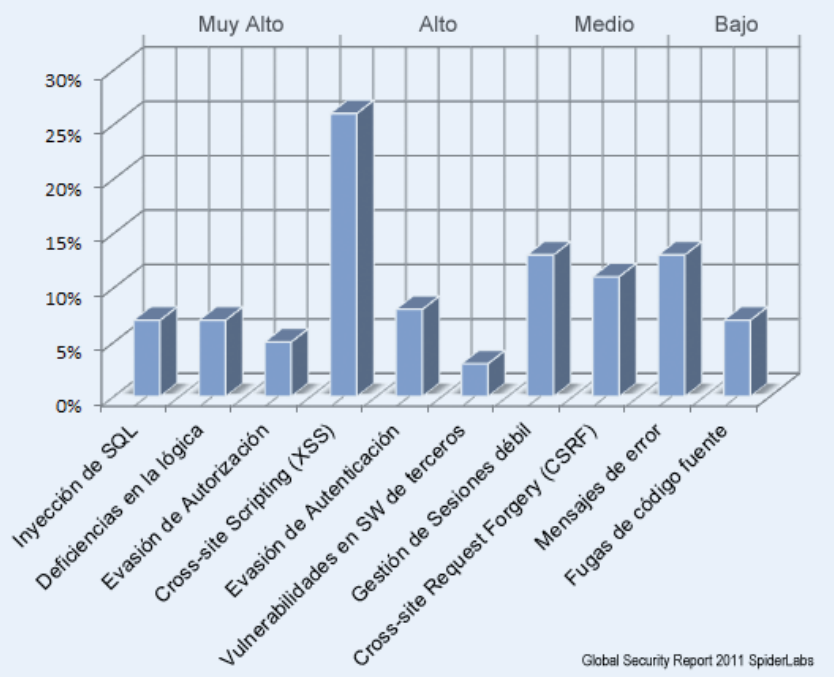
\includegraphics[width=0.9\textwidth]{fig/Vulnerabilidades_OWASP}
      \caption{\small{Tipo de Vulnerabilidades por Impacto~\cite{vulnimpact}}}
		\end{figure}
	\end{column}
	\end{columns}
  \begin{block}{Histórico del riesgo}
    Muchas de estas vulnerabilidades están presentes en el Top 10 de vulnerabilidades OWASP desde 2007 y existen controles que permiten mitigar el riesgo.
  \end{block}
\end{frame}

\begin{frame}[shrink=20]
  \frametitle{Vulnerabilidades recientes en canales cifrados}
  Otro componente en el que se han descubierto múltiples vulnerabilidades críticas son los canales SSL/TLS.
  \begin{center}
    \rowcolors[]{1}{blue!20}{blue!5}
    \begin{tabular}{|l|l|}
      \hline
      {\bf Vulnerabilidad}   			& {\bf Componente afectado}\\
      \hline
      POODLE											&   SSL ver. 3.0        \\
      \hline
      BEAST												&   TLS ver. 1.0        \\
      \hline
      CRIME                       &   TLS compression     \\
      \hline
      BREACH                      &   HTTP compression    \\
      \hline
      Heartbleed                  &   OpenSSL ver. 1.0.1  \\
      \hline
    \end{tabular}
  \end{center}
  \begin{block}{Conclusión}
    La solución, en la mayoría de de los casos, consiste en desactivar las versiones o el componente afectados y el riesgo de afectar la funcionalidad de la plataforma es bajo (dependiendo del entorno).
  \end{block}
\end{frame}

\begin{frame}[allowframebreaks]
  \frametitle{Soluciones.}
  Como respuesta a éstas y otras vulnerabilidades existen múltiples soluciones:
  \begin{itemize}
    \item {\bf Desarrollo de código seguro}: metodologías de desarrollo seguro de aplicaciones, herramientas de análisis de código.
      \par Retos:
      \begin{itemize}
        \item Costes en tiempo y recursos
        \item Conocimiento y herramientas.
        \item Nuevas vulnerabilidades no están consideradas.
      \end{itemize}
    \item {\bf Aplicar un ciclo de vida de aplicaciones}: Aplicar actualizaciones y configuración segura de aplicaciones.
      \par Retos:
      \begin{itemize}
        \item El objetivo es que la aplicación dé servicio. Los demás aspectos son secundarios.
        \item Una actualización puede afectar al entorno.
        \item {\em chmod 777} o {\em iptables -A INPUT -j ACCEPT} funcionan.
      \end{itemize}
    \item {\bf Herramientas de protección perimetral de red}: Firewall de red, Sistema de Prevención de Intrusos.
      \par Reto:
      \begin{itemize}
        \item Desconoce la lógica de aplicación. Lógica limitada a las capas 3 y 4 de red o firmas (cadenas de texto).
        \item Mínima visibilidad con el tráfico cifrado.
      \end{itemize}
    \item {\bf Herramientas de protección perimetral de aplicación.}
      \par Reto: Elevado coste o complejo de mantener.
  \end{itemize}
\end{frame}


\subsection{Estándares y protocolos}
\begin{frame}[shrink=20]
  \frametitle{Estándares y protocolos}
  Existen múltiples iniciativas cuyo objetivo es mejorar la seguridad de las aplicaciones web:
  \begin{itemize}
    \item Metodología del Ciclo de Vida de Desarrollo de Software (\acrshort{sdlc} del inglés).
    \item Estándares como el {\em Payment Card Industry Data Security Standard} (PCI DSS~\cite{pcidssrequirements}).
    \item TLS versión 1.3.
    \item HTTP/2.
    \item TLS Server Name Indication (SNI~\cite{wiki:TLSSNI}).
    \item Security Headers.
  \end{itemize}
  \begin{block}{Uso e implementación}
  Estas Herramientas están disponibles y ofrecen mecanismos válidos para mejorar la seguridad de las plataformas web pero su implementación puede ser compleja o tener un elevado coste.
  \end{block}
\end{frame}

\begin{frame}[shrink=10]
  \frametitle{Uso e implementación}
  Las alternativas implican un coste elevado, implementar soluciones complejas o aceptar el riesgo de seguridad. Y el resultado es el siguiente:
	\begin{columns}
	\begin{column}{0.3\textwidth}
		\begin{figure}
			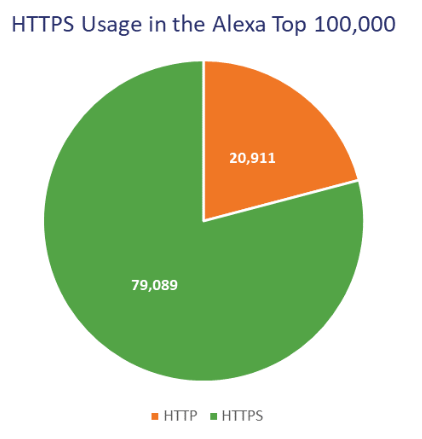
\includegraphics[width=0.9\textwidth]{fig/ImplementationHTTPHTTPS}
      \caption{\small{Tráfico HTTP versus HTTPS ~\cite{thesslstore}}}
		\end{figure}
	\end{column}
	\begin{column}{0.7\textwidth}  %%<--- here
		\begin{figure}
			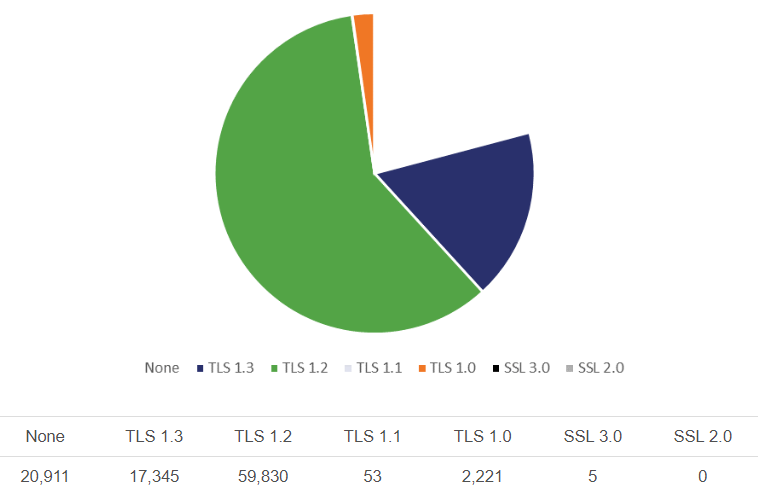
\includegraphics[width=0.7\textwidth]{fig/ImplementationSSLTLS}
      \caption{\small{Máxima versión SSL/TLS soportada~\cite{thesslstore}}}
		\end{figure}
	\end{column}
	\end{columns}
  \begin{block}{Uso e implementación}
  Se ha elegido la versión SSL/TLS como ejemplo de un vector de ataque conocido popularmente cuya mitigación es sencilla.
  \end{block}
\end{frame}

